% ======================================================================================
% CLUSTERING
%

\section{Clustering}

\subsection{PCA}

\begin{table}
	\begin{tabular}{ c c c c c }
		\hline
		\multicolumn{5}{c}{Principal Components} \\ \hline
		-0.51661962 & -0.51137137 &  0.59560332 &  0.29608388 &  0.17086402 \\ \hline
		-0.36102909 &  0.33317829 & -0.15354445 & -0.22331964 &  0.82776969 \\ \hline
		-0.07275141 & -0.28151638 &  0.19427207 & -0.92743392 & -0.13259127 \\ \hline
	\end{tabular}
	\caption{Principal axes in feature space, representing the directions of maximum variance in the data. We can see that the features 3, 5 and 4 are the most variant ones.}
	\label{tab:pca_components}
\end{table}

\begin{table}
	\begin{center}
		\begin{tabular}{cc}
			\hline
			Variance & Ratio \\ \hline
			1.9754988 & 0.39498577 \\
			1.12242609 & 0.22442045 \\
			0.89518261 & 0.17898487 \\
			\hline
		\end{tabular}
		\caption{Variance and ratio for the principal features.}
		\label{tab:pca_variance}
	\end{center}
\end{table}

In table \ref{tab:pca_components} we can see the principle axes for maximum variance in the data after performing PCA set to keep the three most principal components. From this we find that the features that vary the most are in order of variance 3, 5 and 4 that correspond to: ratio between area of grasp and area of object, direction of vector between center of grasp and center of object in y-axis, and the direction of this same vector in the x-axis. In table \ref{tab:pca_variance} we can see the variance for each of these three features as well as their ratio for the dataset. In total these features represent around 80\% of the entire variance, which we set as threshold and we therefore can be content about this new dimensional reduction.

\subsection{K-means}

\begin{figure}
	\begin{subfigure}[b]{\textwidth}
		\input{plot_clustering__mean-silhouette}
		\caption{Mean silhouette coefficient per number of clusters.}
	\end{subfigure}
	\begin{subfigure}[b]{\textwidth}
		\input{plot_clustering__sum-sqr-dist}
		\caption{Sum of squared distances per sample to their closest cluster by number of clusters. Used in the \texttt{elbow method}.}
	\end{subfigure}
	\caption{Mean silhouette coefficient and sum of squared distances per sample to their closest cluster, depending on number of clusters. \texttt{best fit} identifies the possible best number of clusters in accordance to the maximum value of the mean silhouette coefficient and the elbow method.}
	\label{fig:kmeans_score}
\end{figure}

\begin{figure}
	\begin{subfigure}[b]{\textwidth}
		\input{plot_silhouette_5}
		\caption{Silhouette coefficient per sample for five clusters.}
	\end{subfigure}
	\begin{subfigure}[b]{\textwidth}
		\input{plot_silhouette_6}
		\caption{Silhouette coefficient per sample for six clusters.}
		\label{fig:silhouette_6}
	\end{subfigure}
\end{figure}
\begin{figure}
	\ContinuedFloat
	\begin{subfigure}[b]{\textwidth}
		\input{plot_silhouette_7}
		\caption{Silhouette coefficient per sample for seven clusters.}
	\end{subfigure}
	\caption{Silhouette coefficient per sample in each cluster for five, six and seven number of clusters.}
	\label{fig:silhouette_coef}
\end{figure}

\begin{figure}
	\begin{subfigure}[b]{\textwidth}
		\input{plot_clustering__clusters-2d}
		\caption{Two-dimensional representation of the samples and their assigned clusters and centroids.}
	\end{subfigure}
	\begin{subfigure}[b]{\textwidth}
		\input{plot_clustering__clusters-3d}
		\caption{Three-dimensional representation of the samples and their assigned clusters and centroids.}
	\end{subfigure}
	\caption{A two-dimensional and three-dimensional representation of the sample space with their assigned clusters and centroids for six clusters.}
	\label{fig:clusters}
\end{figure}

The results for performing k-means clustering on the transformed data for different numbers of clusters are presented in figure \ref{fig:kmeans_score}. By using the \texttt{elbow method} on the graph containing the sum of squared distances for the samples, we can judge that a number of clusters between five and eight is suitable. With the help of the silhouette score, where six clusters give the best results and falls into this range, we can conclude that six clusters is our best fit.

Figure \ref{fig:silhouette_coef} shows us the silhouette coefficient per sample for the three cases of five, six and seven clusters. We can see that for five clusters there are a lot of samples that have a very poor coefficient in some clusters. Seven has a better repartition but the gradient is quite important for the larger clusters. While six gives us something more balanced, and thus confirming it is a better choice. In figure \ref{fig:silhouette_6} we observe two dominant clusters, the first and third one.

Figure \ref{fig:clusters} show us a two-dimensional and three-dimensional representation of the data divided into clusters and their centers for six clusters. We can notice that it is not entirely obvious how the data is clustered as the data is a bit hard to reduce in dimensionality and visually represent in graphs. However the results for the silhouette scores and elbow method do confirm this clustering.


\subsection{Object cluster assignments}

\begin{figure}
	\input{plot_clustering__obj-sampl-assgmnt}
	\caption{Heatmap over distribution of object samples between clusters.}
	\label{fig:obj_sample_heatmap}
\end{figure}

\begin{table}
	\begin{tabular}{|c|l|}
		\hline
		Cluster & Objects \\
		\hline
		one   & hammer, pen, scalpell, scissors, knife, screwdriver, brush \\
		two   & tube \\
		three & can, pitcher, glass, bottle, cup \\
		four  & box \\
		five  & cutters \\
		six   & - \\
		\hline
	\end{tabular}
	\caption{Cluster assignment of objects between six clusters.}
	\label{tab:object_cluster_assign}
\end{table}

\begin{figure}
	\centering
	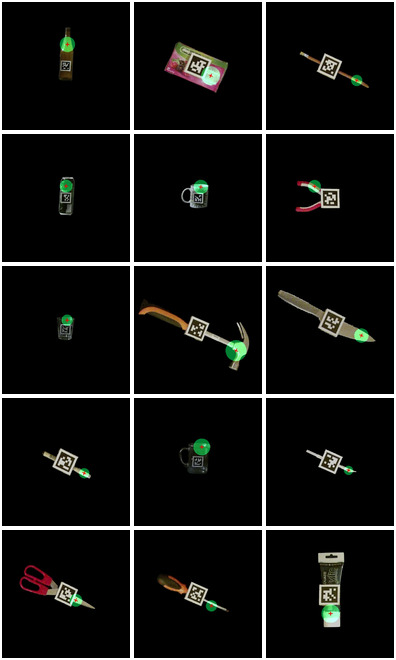
\includegraphics[width=\textwidth]{img/results/objects.jpg}
	\caption{The training objects with the mean values of the corresponding cluster applied to them.}
	\label{fig:results_objects}
\end{figure}

Figure \ref{fig:obj_sample_heatmap} represents a heatmap over the distribution of samples belonging to each object between the clusters. We can see that each cluster represents at least one object, with the exception of the third cluster. The screwdriver, knife, scissors, pen, hammer, scalpell and brush have the largest majority of their samples belonging to the first cluster, while the bottle, pitcher, glass, cup and can are represented by the fourth cluster. The cutters, box and tube are represented by their own clusters, respectively sixth, second and fifth clusters, showing that they are handed over in unique ways compared to the other previous objects. The third cluster seems quite evenly distributed over the objects, with the pitcher having the largest part, which indicates that it can be considered as a cluster of noise from the input data. Table \ref{tab:object_cluster_assign} shows us the final distribution of the objects between the clusters. In figure \ref{fig:results_objects} every object is visualized with their corresponding cluster mean features applied to them.

Already here we can see some similarities between the objects that are clustered together, notable in clusters one and four. The first one includes objects that are longer and thinner and that often include a tip of contact for its usage, like the head of the hammer or the tip of the brush. While the fourth cluster is made of objects that are larger and cylindrical, often used for containing fluids which explains they need to be held similar fashion when handed over as to not spill out the contents.



% ======================================================================================
% CLASSIFICATION
%

\section{Classification}

\subsection{Network configuration}
\label{sec:res_setup}

To summarize the clustering part of this work we are able to divide the objects used for training into a total of five classes. An issue with these results is that three of the classes are represented by a sole item. We judge that it would not be possible to create a balanced dataset to represent equally each class this way. It would also defeat the purpose as to create a model that no longer identifies single object classes, but instead visually similar objects within a same class. Therefore we will discard these three classes and concentrate on the two classes that contain multiple objects. Our network will then be trained for two outputs through a softmax layer.

\begin{table}
	\begin{tabular}{|c|p{5cm}|p{5cm}|}
		\hline
		Class & Training objects & Test objects \\
		\hline
		one & hammer, pen, scalpell, scissors, knife, screwdriver, brush & scissors, fork, knife, spoon, spatula, wooden spoon \\
		\hline
		two & can, pitcher, glass, bottle, cup & bottle, carafe, glass, cup, wine glass, beer glass \\
		\hline
	\end{tabular}
	\caption{Overview of objects included in training set and test set.}
	\label{tab:classification_objects}
\end{table}

In section \ref{sec:testing} we gave a list of objects that are to be used for testing. These were chosen after we made the decision regarding outputs for the network to achieve a balanced dataset over the outputs for testing. Table \ref{tab:classification_objects} shows the distribution of the test objects into classes with the corresponding training objects.


\subsection{Finetuning the network}

\begin{figure}
	\centering
	\begin{subfigure}[b]{\textwidth}
		\input{plot_classification__results-loss}
		\caption{Loss.}
		\label{fig:results_plots_loss}
	\end{subfigure}
	\begin{subfigure}[b]{\textwidth}
		\input{plot_classification__results-val}
		\caption{Validation accuracy.}
		\label{fig:results_plots_val}
	\end{subfigure}
\end{figure}
\begin{figure}
	\ContinuedFloat
	\begin{subfigure}[b]{\textwidth}
		\input{plot_classification__results-test}
		\caption{Test accuracy.}
		\label{fig:results_plots_test}
	\end{subfigure}
	\label{fig:results_plots}
	\caption{Cross entropy, validation and test accuracy during training of the model.}
\end{figure}

\begin{figure}
	\input{plot_classification__confmat}
	\caption{Confusion matrix for k=1.}
	\label{fig:confusion_matrix}
\end{figure}

\begin{table}
	\centering
	\begin{tabular}{l | c | c | c | c}
		\hline
		Set        & Min   & Max   & Mean  & Std.  \\ \hline
		Validation & 0.992 & 1.0   & 0.998 & 0.003 \\
		Test       & 0.886 & 0.922 & 0.906 & 0.013 \\
		\hline
	\end{tabular}
	\caption{Accuracy on the training and test objects for 5 fold cross validation.}
	\label{tab:results_accuracy}
\end{table}

\begin{table}
	\centering
	\begin{tabular}{l | c | c | c | c}
		\hline
		Object       & Min   & Max   & Mean  & Std.  \\ \hline
		Beerglass    & 0.821 & 0.905 & 0.864 & 0.032 \\
		Bottle       & 1.000 & 1.000 & 1.000 & 0.000 \\
		Carafe       & 0.596 & 0.730 & 0.674 & 0.057 \\
		Cup          & 1.000 & 1.000 & 1.000 & 0.000 \\
		Fork         & 1.000 & 1.000 & 1.000 & 0.000 \\
		Glass        & 0.827 & 0.988 & 0.901 & 0.064 \\
		Knife        & 1.000 & 1.000 & 1.000 & 0.000 \\
		Scissors     & 1.000 & 1.000 & 1.000 & 0.000 \\
		Spatula      & 0.940 & 0.964 & 0.955 & 0.009 \\
		Spoon        & 0.976 & 1.000 & 0.993 & 0.010 \\
		Wineglass    & 0.471 & 0.644 & 0.538 & 0.059 \\
		Wooden spoon & 0.926 & 1.000 & 0.951 & 0.027 \\
		\hline
	\end{tabular}
	\caption{Accuracy on individual objects in the test set for 5 fold cross validation.}
	\label{tab:results}
\end{table}

\begin{table}
	\centering
	\begin{tabular}{l | c | c | c}
		\hline
		Class & Precision & Recall & \(F_1\) score \\ \hline
		A     & 0.875     & 0.994  & 0.931 \\
		B     & 0.991     & 0.841  & 0.910 \\ \hline
	\end{tabular}
	\caption{Precision, Recall and \(F_1\) score for the classes.}
	\label{tab:results_precision_recall_f1}
\end{table}


Considering the limited amount of objects that we are using for training the network we run a high risk of overfitting it to these specific objects, and it will not properly classify new ones even though similar. We want the network to recognize the objects in the training set in an abstract fashion as to not learn too much detail about the individual objects. For finetuning the network we therefore chose to train using a larger batch size of 128 and learning rate of 0.0001 for 20 epochs, keeping the initial value of 0.5 for dropout that was used when training the initial weights.

We can see from figure \ref{fig:results_plots_loss} that the network very quickly is able to find zero loss and validation accuracy above 99\%, it however struggles to become steady on the test accuracy. We suspect that is due to some unfortunate overfitting to the training set because we can notice a slight correlation between a lower validation accuracy and higher test accuracy. The graphs for accuracy are also quite irregular between the runs. There is a chance that because of the limitations in data set the network becomes very sensitive to the order that the input is beeing fed for training.

Figure \ref{fig:confusion_matrix} shows us the confusion matrix for the network when it achieved its highest test accuracy of 92.2\% and validation accuracy of 100\%. We obtain a precision of 0.875, recall of 0.994 and an \(F_1\) score of 0.931 for class \(A\) and a precision of 0.992, recall of 0.841 and a \(F_1\) score of 0.91 for class \(B\) (summarized in table \ref{tab:results_precision_recall_f1}). The results tell us that the network is in the end, despite otherwise good results, a little biased towards the first class. This can be explained by the fact that even though the training set is balanced between the classes in terms of number of images per class, it is however not balanced in the number of objects. The first class represents seven objects while the second one only five, meaning that there are more versatile features to learn for the one class than the other.


\begin{figure}
	\centering
	\begin{subfigure}[b]{0.3\textwidth}
		\includegraphics[width=\textwidth]{img/results/bad-images/new-beerglass_100_80.jpg}
		\caption{Beer glass.}
	\end{subfigure}
	\begin{subfigure}[b]{0.3\textwidth}
		\includegraphics[width=\textwidth]{img/results/bad-images/new-carrafe_102_53.jpg}
		\caption{Carafe.}
	\end{subfigure}
	\begin{subfigure}[b]{0.3\textwidth}
		\includegraphics[width=\textwidth]{img/results/bad-images/new-glass_105_43.jpg}
		\caption{Glass}
	\end{subfigure}
	\begin{subfigure}[b]{0.3\textwidth}
		\includegraphics[width=\textwidth]{img/results/bad-images/new-spatula_108_36.jpg}
		\caption{Spatula}
		\label{fig:results_bad_images__spatula}
	\end{subfigure}
	\begin{subfigure}[b]{0.3\textwidth}
		\includegraphics[width=\textwidth]{img/results/bad-images/new-spoon_109_100.jpg}
		\caption{Spoon.}
		\label{fig:results_bad_images__spoon}
	\end{subfigure}
	\begin{subfigure}[b]{0.3\textwidth}
		\includegraphics[width=\textwidth]{img/results/bad-images/new-wineglass_110_22.jpg}
		\caption{Wine glass.}
	\end{subfigure}
	\begin{subfigure}[b]{0.3\textwidth}
		\includegraphics[width=\textwidth]{img/results/bad-images/new-woodenspoon_111_31.jpg}
		\caption{Wooden spoon.}
		\label{fig:results_bad_images__wooden_spoon}
	\end{subfigure}
	\caption{Some images with incorrect predictions.}
	\label{fig:results_bad_images}
\end{figure}


In figure \ref{fig:results_bad_images} we show a sample image of each object that did not achieve 100\% accuracy (a larger sample set can be found in appendix \ref{app:bad_images}). We can observe that the network struggles with objects that are made of glass, especially transparent and thinner glass. This is the case for the carafe, wine glass and beer glass. Other objects in the same class that are not as transparent such as the bottle and the cup, do not have this problem though, and can achieve accuracies of 100\%. This is probably due to the noise and artifacts that appear in the images taken with the depth camera for objects made of thin glass and also the fact they do not have any distinct color they almost become seemingly invisible in some images making them very challenging to identify. Objects in class \(A\) are in one hand quite small in comparison, the network might associate the amount of visible background to this class and when unsure classifying objects that are quite transparent to this class instead. The training set is probably not representative enough of these kind of objects for it to properly learn features to help distinguish them.

A special case is the wine glass, that has the poorest results. Besides the fact that it presents the same challenges as the other glass objects its geometry is also something of a combination of the two classes. Though it has a cylindrical part for liquids it also has a long and thin handle that is similar to for example a pen or brush. As no object in the training set is of the same complex geometry the network as a result has a hard time predicting the correct class for the wineglass.

From the first class there are some objects that did not achieve 100\% accuracy either. From the images of the spatula and the spoon (figures \ref{fig:results_bad_images__spoon} and \ref{fig:results_bad_images__spatula}) there is no object in the other class that we can think that the network confused the objects with, however there is a large amount of noise in these images. We can suspect that the network has learned to associate a degree of noise that is very common in images for glass objects with the second class. On the other hand there are some incorrect predictions that might not always be due to the image quality, as for example the wooden spoon (figure \ref{fig:results_bad_images__wooden_spoon}). One theory to why some of the images of the wooden spoon were incorrectly predicted is that it has some resemblence due to color to the bottle that the network was trained on which is of the opposite class. This shows the limitations of training on such a small dataset of objects that are not versatily represented.


\subsection{Object impact on accuracy}
\label{sec:obj_impact}

\begin{table}
	\centering
	\begin{tabular}{l | l}
		\hline
		Pair  & Objects \\ \hline
		one   & glass, hammer \\
		two   & bottle, knife \\
		three & can, scissors \\
		four  & pitcher, brush \\
		five  & cup, screwdriver \\
		\hline
	\end{tabular}
	\caption{Pairs of objects in order they are added to the training set.}
	\label{tab:obj_pairs}
\end{table}

\begin{table}
	\centering
	\begin{tabular}{l | p{8cm}}
		\hline
		\# objects in training set & Objects \\ \hline
		two   & glass, hammer \\
		four  & glass, hammer, bottle, knife \\
		six   & glass, hammer, bottle, knife, can, scissors \\
		eight & glass, hammer, bottle, knife, can, scissors, pitcher, brush \\
		ten   & glass, hammer, bottle, knife, can, scissors, pitcher, brush, cup, screwdriver \\
		\hline
	\end{tabular}
	\caption{Objects contained in the corresponding training sets.}
	\label{tab:obj_training_sets}
\end{table}

We will explore the effects the size of the training set, as well as the individual objects, have on the final test accuracy. This section will be dedicated to presenting results from training the network on different sizes of training sets. This is done by splitting the objects into pairs (one per class) and then training the network on the subset and measuring its accuracy on the test set. After each training session, a new pair of objects is added to the training set and we repeat this until all objects are in the training set. We keep the same learning parameters as in the previous section with a batch size of 128, a learning rate of 0.0001 and a dropout of 0.5\% for 20 epochs.

Table \ref{tab:obj_pairs} summarizes which pairs of objects that were created and the order they were added to the training set, and for clarification table \ref{tab:obj_training_sets} summarizes the objects that are used for each training session. These pairs were chosen randomly. Note that there are only ten objects in total for this test (five for each class), but we have twelve in total. This is because the dataset is not balanced on objects between classes so we chose to discard two: the \texttt{scalpel} and the \texttt{pen}. These last two objects were chosen to be removed because they have very similar features that are shared with and represented in the dataset through the \texttt{brush} and in some ways the \texttt{screwdriver}.

A more thourough method would be to test all possible permutations of objects for training and evaluation, but this would be quite time consuming. We therefore rely on this test to give us accurate enough ideas about the impact of each object.


\begin{table}
	\centering
	\begin{tabular}{l | l | c | c | c | c}
		\hline
		\# objects in training set & Set & Min & Max & Mean & Std. \\ \hline

		two
		& Validation & 0.989 & 1.0   & 0.998 & 0.005 \\
		& Test       & 0.806 & 0.864 & 0.841 & 0.023 \\ \hline

		four
		& Validation & 1.0   & 1.0   & 1.0   & 0.000 \\
		& Test       & 0.825 & 0.900 & 0.852 & 0.039 \\ \hline

		six
		& Validation & 0.992 & 1.0   & 0.997 & 0.003 \\
		& Test       & 0.835 & 0.925 & 0.880 & 0.038 \\ \hline

		eight
		& Validation & 0.995 & 1.0   & 0.998 & 0.003 \\
		& Test       & 0.940 & 0.956 & 0.944 & 0.007 \\ \hline

		ten
		& Validation & 0.996 & 1.0   & 0.998 & 0.001 \\
		& Test       & 0.936 & 0.978 & 0.961 & 0.016 \\ \hline
	\end{tabular}
	\caption{Validation and test accuracy for 5 fold cross validation.}
	\label{tab:results_perobj}
\end{table}

\begin{figure}
	\input{plot_classification__object-impact}
	\caption{Evolution of validation and test accuracy as a factor of number of object in training set.}
	\label{fig:object_impact}
\end{figure}

\begin{figure}
	\input{plot_classification__object-impact_object}
	\caption{Accuracy for each object depending on how many objects the network is trained on.}
	\label{fig:object_impact_heatmap}
\end{figure}

The results for each session are reported in table \ref{tab:results_perobj}. In figure \ref{fig:object_impact} we present the evolution of the test and validation accuracy when adding new objects to the training set, which is also summarized per object in figure \ref{fig:object_impact_heatmap}. In the end we achieve a model with a mean test accuracy of 96.1\% with a standard deviation of 1.6\% and a validation accuracy of 99.8\% with a standard deviation of 0.1\%.

In overall we can see that the network performs quite well for all sizes of the training set. Lowest is of course when training for only two objects, the \texttt{hammer} and the \texttt{glass} with a mean test accuracy of 84.1\% and standard deviation of 2.3\%. Validation accuracy for all sessions is steady between 99.7\% and 100\%. But even then there are only two objects that have very low accuracy, while all others have near perfect accuracy between 96-100\%. Even the wineglass that the network usually struggles with has an accuracy of 100\%. The two objects in question here with very low accuracy are the \texttt{bottle} and the \texttt{cup}. This comes though as little surprise as they have very little similarities with the \texttt{glass} which is the representative of their common class, their shapes are not quite similar and they have more in common with the \texttt{hammer} according to their color.

As soon as two more objects are added for training the performance for these objects directly becomes perfect. The \texttt{bottle} helps with both shape and color to group the two outliers from the previous session. However there is only a very slight increase to the overall performance of the network, as it becomes more confused over the other objects. With some small exceptions the accuracy of the network only increases for each object when adding a new pair to the training set. By looking at the curve for the test accuracy in figure \ref{fig:object_impact} we notice that the increase is quite steady per pair added. We however observe the exceptional largest increase in performance when introducing the fourth pair of objects, the \texttt{picther} and \texttt{brush}. Objects that benefit from it the most are the ones made of glass suggesting it is good with more representative features of transparent glass for the network to learn.

We can conclude the results for the tests in this section with the hypothesis that increasing the training set only benefits the overall performance of the network. Our results suggest that the network performance can increase further with a larger dataset, but we are limited to the objects that we have at our disposal. We also see the importance of adding objects that are difficult to classify, such as those made of glass in our case, which give the greatest addition to the accuracy.

A last observation that we can make in this section is that the final performance of the network, after trained with five pairs of objects is actually better than the accuracy reported in the previous section. As mentioned before the classes are not balanced in number of objects, however the training sets are in terms of number of images per class. We conclude that it is therefore very important that we also balance in number of objects. Here we chose manually the objects to discard. It would require more work to test if this choice was the best and then to develop an algorithm for the system to do this by itself, which is why this method was not adopted earlier.
